% Options for packages loaded elsewhere
\PassOptionsToPackage{unicode}{hyperref}
\PassOptionsToPackage{hyphens}{url}
\PassOptionsToPackage{dvipsnames,svgnames,x11names}{xcolor}
\documentclass[
  10pt,
  fontset=fandol]{ctexart}
\usepackage{xcolor}
\usepackage[margin=16mm]{geometry}
\usepackage{amsmath,amssymb}
\setcounter{secnumdepth}{-\maxdimen} % remove section numbering
\usepackage{iftex}
\ifPDFTeX
  \usepackage[T1]{fontenc}
  \usepackage[utf8]{inputenc}
  \usepackage{textcomp} % provide euro and other symbols
\else % if luatex or xetex
  \usepackage{unicode-math} % this also loads fontspec
  \defaultfontfeatures{Scale=MatchLowercase}
  \defaultfontfeatures[\rmfamily]{Ligatures=TeX,Scale=1}
\fi
\usepackage{lmodern}
\ifPDFTeX\else
  % xetex/luatex font selection
\fi
% Use upquote if available, for straight quotes in verbatim environments
\IfFileExists{upquote.sty}{\usepackage{upquote}}{}
\IfFileExists{microtype.sty}{% use microtype if available
  \usepackage[]{microtype}
  \UseMicrotypeSet[protrusion]{basicmath} % disable protrusion for tt fonts
}{}
\makeatletter
\@ifundefined{KOMAClassName}{% if non-KOMA class
  \IfFileExists{parskip.sty}{%
    \usepackage{parskip}
  }{% else
    \setlength{\parindent}{0pt}
    \setlength{\parskip}{6pt plus 2pt minus 1pt}}
}{% if KOMA class
  \KOMAoptions{parskip=half}}
\makeatother
\usepackage{graphicx}
\makeatletter
\newsavebox\pandoc@box
\newcommand*\pandocbounded[1]{% scales image to fit in text height/width
  \sbox\pandoc@box{#1}%
  \Gscale@div\@tempa{\textheight}{\dimexpr\ht\pandoc@box+\dp\pandoc@box\relax}%
  \Gscale@div\@tempb{\linewidth}{\wd\pandoc@box}%
  \ifdim\@tempb\p@<\@tempa\p@\let\@tempa\@tempb\fi% select the smaller of both
  \ifdim\@tempa\p@<\p@\scalebox{\@tempa}{\usebox\pandoc@box}%
  \else\usebox{\pandoc@box}%
  \fi%
}
% Set default figure placement to htbp
\def\fps@figure{htbp}
\makeatother
\setlength{\emergencystretch}{3em} % prevent overfull lines
\providecommand{\tightlist}{%
  \setlength{\itemsep}{0pt}\setlength{\parskip}{0pt}}
\usepackage{amsmath,amssymb,mathtools,needspace}
\xeCJKDeclareCharClass{CJK}{"2032,"0400->"04FF,"2160->"216B,"2460->"2473,"25A0,"25C7,"25CB,"25CF}
\IfFontExistsTF{Arial Unicode MS}{\xeCJKsetup{AutoFallBack=true}\setCJKfallbackfamilyfont{\CJKrmdefault}{Arial Unicode MS}}{}
\setcounter{secnumdepth}{0}
\setlength{\emergencystretch}{2em}
\allowdisplaybreaks
\usepackage{bookmark}
\IfFileExists{xurl.sty}{\usepackage{xurl}}{} % add URL line breaks if available
\urlstyle{same}
\hypersetup{
  pdftitle={多项式插值的问题},
  colorlinks=true,
  linkcolor={Maroon},
  filecolor={Maroon},
  citecolor={Blue},
  urlcolor={Blue},
  pdfcreator={LaTeX via pandoc}}

\title{多项式插值的问题}
\author{}
\date{}

\begin{document}
\maketitle

\subsubsection{2.7.1 多项式插值的问题}\label{ux591aux9879ux5f0fux63d2ux503cux7684ux95eeux9898}

根据区间 \([a,b]\) 上给出的节点构造插值多项式 \(L_n(x)\) 近似 \(f(x)\) 时，人们往往认为 \(L_n(x)\) 的次数 \(n\) 越高逼近 \(f(x)\) 的精度越好，但实际上并非如此。这是因为，对于任意的插值节点，当 \(n\to\infty\) 时，\(L_n(x)\) 不一定收敛到 \(f(x)\)。20 世纪初 Runge 就给出了一个等距节点插值多项式 \(L_n(x)\) 不收敛到 \(f(x)\) 的例子：考察函数 \(f(x)=1/(1+x^2)\)，它在 \([-5,5]\) 上各阶导数均存在，但在 \([-5,5]\) 上取 \(n+1\) 个等距节点

\[x_k=-5+10\frac{k}{n}\quad(k=0,1,\cdots,n)\]

所构造的 Lagrange 插值多项式

\begin{quote}
续页：该多项式和 Runge 现象见下一页。
\end{quote}

\href{../../source-images/pdf-046.jpeg}{查看原页}

\begin{quote}
本页接上页 2.7.1 正文。
\end{quote}

\[L_n(x)=\sum_{j=0}^n\frac{1}{1+x_j^2}\frac{\omega_{n+1}(x)}{(x-x_j)\omega'_{n+1}(x_j)}\]

当 \(n\to\infty\) 时只在 \(|x|\leqslant3.63\) 内收敛，而在这区间外是发散的。

下面取 \(n=10\)，根据计算画出 \(y=L_{10}(x)\) 及 \(y=1/(1+x^2)\) 在 \([-5,5]\) 上的图形，如图 2.5 所示。

从图 2.5 可看到，在 \(x=\pm5\) 附近 \(L_{10}(x)\) 与 \(f(x)=1/(1+x^2)\) 偏离很远，例如，\(L_{10}(4.8)=1.804\,38,f(4.8)=0.041\,60\)。这说明用高次插值多项式 \(L_n(x)\) 近似 \(f(x)\) 效果并不好，因而通常不用高次插值，而用低次插值。从该例看到，如果把 \(y=1/(1+x^2)\) 在节点 \(x=0,\allowbreak \pm1,\allowbreak \pm2,\allowbreak \pm3,\allowbreak \pm4,\allowbreak \pm5\) 处用折线连起来，显然比 \(L_{10}(x)\) 逼近 \(f(x)\) 好得多。这正是下面要讨论的分段低次插值的出发点。

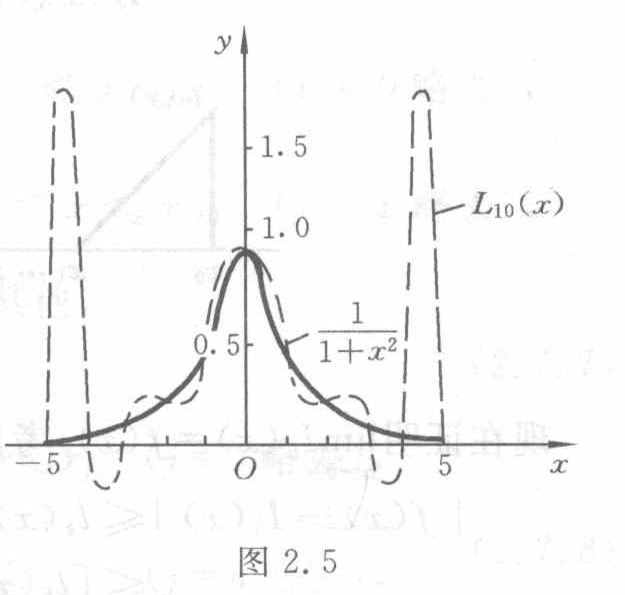
\includegraphics[width=0.85\linewidth,height=\textheight,keepaspectratio,alt={图 2.5（原图裁切）}]{../assets/ch02b/figure-2-5.png}

\begin{quote}
图 2.5（原图）：横轴 \(x\)，纵轴 \(y\)，原点 \(O\)；横轴标有 \(-5,5\)，纵轴标有 \(0.5,1.0,1.5\)。两条曲线标签为 \(L_{10}(x)\) 与 \(\frac{1}{1+x^2}\)。虚线插值曲线在两端附近出现明显振荡。
\end{quote}

\begin{center}\rule{0.5\linewidth}{0.5pt}\end{center}

\subsection{相关原页校注（agent 补充）}\label{ux76f8ux5173ux539fux9875ux6821ux6ce8agent-ux8865ux5145}

以下校注来自本节覆盖的原页，可能也涉及同页相邻小节；原文照录与校正说明分开保留。

\subsubsection{原书 PDF 页 46 的校注}\label{ux539fux4e66-pdf-ux9875-46-ux7684ux6821ux6ce8}

\href{../pages/pdf-046.md}{完整原页转录} · \href{../../source-images/pdf-046.jpeg}{原页图像}

校注记录：ch02b-E001。

\begin{quote}
\textbf{校注（agent 补充；原书疑误）}：式（2.7.3）第二分支原扫描确为 \(\frac{x_j-x_{j+1}}{x-x_{j+1}}\)，此处已原样保留，参见\href{../assets/ch02b/pdf-046-eq-2-7-3-detail.png}{原式放大裁图}。该式在 \(x=x_{j+1}\) 处分母为零，与本页分段线性、连续性及 \(l_j(x_{j+1})=0\) 的条件矛盾。按这些条件，第二分支应为 \(\frac{x-x_{j+1}}{x_j-x_{j+1}}\)。这属于原书疑误，区别于 OCR 另将分母误识为 \(x_j-x_{j+1}\)。
\end{quote}

\subsection{本节覆盖原页的校注记录}\label{ux672cux8282ux8986ux76d6ux539fux9875ux7684ux6821ux6ce8ux8bb0ux5f55}

下列记录按原页关联，含同页相邻小节的校注；计算时同时读取上文校注和完整原页。

\begin{itemize}
\tightlist
\item
  \texttt{ch02b-E001}：原书 PDF 页 46
\end{itemize}

\end{document}
